
\label{chap:sepsis}
\section{Sepsis and Vasomotion}

Sepsis is a condition, which develops through systemic inflammatory response syndrome (SIRS) with presence of an infection or bacteria within the body. Sepsis adversely affect heart rate, blood pressure, oxygen extraction and body temperature and leads to multi organ failure in worst cases.\cite{pluta2010,kanta2014}

Since sepsis is based on an inflammation, the body activates the inflammatory cascade as an immune response. Some factors released by the inflammatory cascade have influence on vasodilation and triggers a dispersed systemic vasodilation and decrease the responsiveness of the affected vasculature. It is known that sepsis leads to imbalance of the microcirculation, whereby the blood distribution becomes unequal. Areas with a lack of blood supply which already have a need of blood might get less blood, whereas areas with sufficient supply might get more of the available amount of blood. As an adequate oxygen supply requires a sufficient circulation, the condition of the areas with a lack of blood supply deteriorates.
If local microcirculation of several organs like kidneys or liver is impaired over time, it leads to failure of these organs.\cite{baudouin2008,kanta2014}

The vascular endothelium is affected within the incidents of sepsis, because the stressful environments of sepsis activate vascular endothelial cells. Normally it is a protective response, but in sepsis where the disorder remains, this response exaggerates unpredictably. The endothelial probity get lost and causes cell injury and hypoxia. Moreover the tissue underlying the capillaries suffer from the obstructed capillary perfusion and related hypoxia. The scheme in figure \ref{fig:Sepsis} shows the role of vascular endothelium on the way to organ failure.\cite{baudouin2008}

\begin{figure}[H]
	\centering	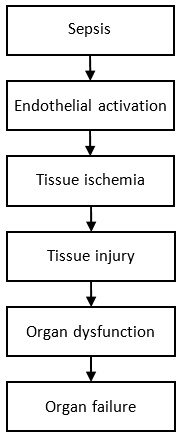
\includegraphics[width=0.2\textwidth]{figures/SepsisEndo}
	\caption{Scheme that shows the progression from sepsis to organ failure. Modified from \cite{baudouin2008}.}
	\label{fig:Sepsis}
\end{figure}

Summarized, sepsis affects the processes within the microcirculation to an extent that the impairment exceed the autoregulation abilities of vasomotion.